\documentclass{beamer}

\usepackage{algorithm}
\usepackage{algpseudocode}
\usepackage{soul}
\usepackage{subcaption}
\usepackage{tikz}
\usetikzlibrary{arrows,fit,petri,topaths}
\usepackage{tkz-berge}

% theme
\usetheme{ccc}

% colors
\definecolor{tcolorboxGray}{RGB}{243,243,243}
\definecolor{LightGray}{RGB}{230,230,230}
\definecolor{MediumGray}{RGB}{179,179,179}
\definecolor{DarkGray}{RGB}{128,128,128}
\definecolor{LightRed}{RGB}{255,213,213}
\definecolor{MediumRed}{RGB}{255,128,128}

\newcommand{\includeressource}[2][]{\includegraphics[#1]{../resources/pdf/#2}}
\newcommand{\inputressource}[1]{\input{../resources/tex/#1}}

\begin{document}

\title{Faster MPSoC Task Mapping via\\Symmetry Reduction}
\author{Timo Nicolai\\\texttt{timo.nicolai@mailbox.tu-dresden.de}}

\begin{frame}
\titlepage
\end{frame}

\begin{frame}
  \frametitle{Problem Statement}

  \begin{center}
    \includeressource[width=.5\linewidth]{regular_mesh_m_n.pdf}
  \end{center}
\end{frame}

\begin{frame}
  \frametitle{Problem Statement}

  \begin{center}
    \includeressource[width=.3\linewidth]{regular_mesh_m_n.pdf}
  \end{center}

  \begin{itemize}
    \item<1-> Want to intelligently map tasks to processing elements
    \item<2-> Best choice depends on underlying optimality criteria
    \item<3-> Need to perform costly simulation!
  \end{itemize}
\end{frame}

\begin{frame}
  \frametitle{Symmetry Reduction}

  \begin{itemize}
    \setlength\itemsep{.25cm}
    %
    \item<1-> One approach:
      \begin{itemize}
        \item<1-> Generate promising mappings based on previous simulations
        \item<2-> $\rightarrow$ Traverse search space ``intelligently''
      \end{itemize}
    \item<3-> Another approach:
      \begin{itemize}
        \item<3-> Partition search space \textit{by (partial) symmetry}
        \item<4-> Only work with representative of each partition
        \item<5-> $\rightarrow$ ``Collapse'' search space
       \end{itemize}
    \item<6-> Both approaches can be combined!
  \end{itemize}
\end{frame}

\begin{frame}
  \frametitle{Symmetry Reduction}

  \begin{figure}
    \centering
    %
    \begin{subfigure}{.3\textwidth}
      \begin{overprint}
        \onslide<1>\includeressource[width=\textwidth]{%
          regular_mesh_4_4_mapping1_noarrow.pdf}
        \onslide<2>\includeressource[width=\textwidth]{%
          regular_mesh_4_4_mapping1.pdf}
      \end{overprint}
    \end{subfigure}
    %
    \hspace*{.5cm}
    %
    \begin{subfigure}{.3\textwidth}
      \includeressource[width=\textwidth]{regular_mesh_4_4_mapping2.pdf}
    \end{subfigure} \\
    %
    \vspace*{.5cm}
    %
    \begin{subfigure}{.3\textwidth}
      \includeressource[width=\textwidth]{regular_mesh_4_4_mapping4.pdf}
    \end{subfigure}
    %
    \hspace*{.5cm}
    %
    \begin{subfigure}{.3\textwidth}
      \begin{overprint}
        \onslide<1>\includeressource[width=\textwidth]{%
          regular_mesh_4_4_mapping5_noarrow.pdf}
        \onslide<2>\includeressource[width=\textwidth]{%
          regular_mesh_4_4_mapping5.pdf}
      \end{overprint}
    \end{subfigure}
  \end{figure}
\end{frame}

\begin{frame}
  \frametitle{Inspirations and Contributions}

  \begin{itemize}
    \setlength\itemsep{.25cm}

    \item<1-> Original idea: \cite{Goens}
    \item<2-> Theoretical foundations: \cite{Holt} and \cite{Mitchell}
    \item<3-> Important optimizations: \cite{Donaldson}
    \item<4-> Resulting framework: \cite{mpsym}
  \end{itemize}
\end{frame}

\begin{frame}
  \frametitle{Representing Symmetries:\\Automorphism Groups}

  \only<1>{
    \begin{figure}
      \centering
      %
      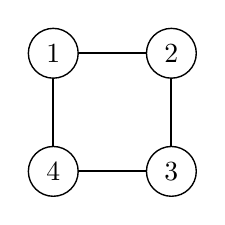
\begin{tikzpicture}
        % vertices
        \Vertex[x=0,y=0,L=$1$]{1}
        \Vertex[x=1.5,y=0,L=$2$]{2}
        \Vertex[x=1.5,y=-1.5,L=$3$]{3}
        \Vertex[x=0,y=-1.5,L=$4$]{4}
        % edges
        \Edge(1)(2)
        \Edge(2)(3)
        \Edge(3)(4)
        \Edge(4)(1)
      \end{tikzpicture}
    \end{figure}
  }

  \only<2>{
    \begin{figure}
      \centering
      %
      \begin{subfigure}{.2\paperwidth}
        \centering
        %
        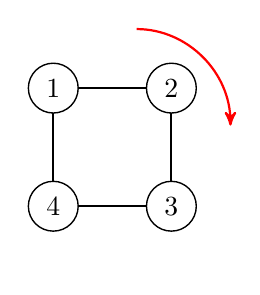
\begin{tikzpicture}[baseline=(current bounding box.center)]
          % vertices
          \Vertex[x=0,y=0,L=$1$]{1}
          \Vertex[x=1.5,y=0,L=$2$]{2}
          \Vertex[x=1.5,y=-1.5,L=$3$]{3}
          \Vertex[x=0,y=-1.5,L=$4$]{4}
          % edges
          \Edge(1)(2)
          \Edge(2)(3)
          \Edge(3)(4)
          \Edge(4)(1)
          % arrow
          \Vertex[empty,x=1,y=0.75]{x}
          \Vertex[empty,x=2.25,y=-0.5]{y}
          \tikzstyle{EdgeStyle}=[post, bend angle=45, bend left, style=thick]
          \Edge[color=red](x)(y)
          % dummy
          \Vertex[empty,x=1,y=-2.25]{x}
        \end{tikzpicture}
      \end{subfigure}
      %
      \Large$\Rightarrow$\normalsize
      %
      \begin{subfigure}{.2\paperwidth}
        \centering
        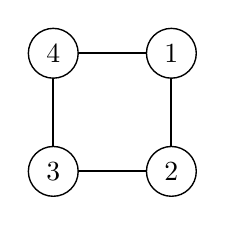
\begin{tikzpicture}[baseline=(current bounding box.center)]
          % vertices
          \Vertex[x=0,y=0,L=$4$]{1}
          \Vertex[x=1.5,y=0,L=$1$]{2}
          \Vertex[x=1.5,y=-1.5,L=$2$]{3}
          \Vertex[x=0,y=-1.5,L=$3$]{4}
          % edges
          \Edge(1)(2)
          \Edge(2)(3)
          \Edge(3)(4)
          \Edge(4)(1)
        \end{tikzpicture}
      \end{subfigure}
      %
      \Large$\Rightarrow$\normalsize\makebox[.2\paperwidth]{$\ (1\ 2\ 3\ 4)$\hfill}
      %
      \begin{subfigure}{.2\paperwidth}
        \centering
        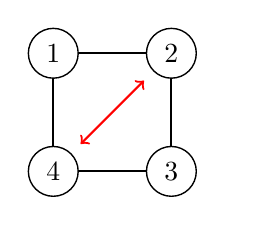
\begin{tikzpicture}[baseline=(current bounding box.center)]
          % vertices
          \Vertex[x=0,y=0,L=$1$]{1}
          \Vertex[x=1.5,y=0,L=$2$]{2}
          \Vertex[x=1.5,y=-1.5,L=$3$]{3}
          \Vertex[x=0,y=-1.5,L=$4$]{4}
          % edges
          \Edge(1)(2)
          \Edge(2)(3)
          \Edge(3)(4)
          \Edge(4)(1)
          % arrow
          \tikzstyle{EdgeStyle}=[pre and post, shorten <=5pt,shorten >=5pt, style=thick]
          \Edge[color=red](2)(4)
          % dummy
          \Vertex[empty,x=2.25,y=-0.75]{x}
        \end{tikzpicture}
      \end{subfigure}
      %
      \Large$\Rightarrow$\normalsize
      %
      \begin{subfigure}{.2\paperwidth}
        \centering
        %
        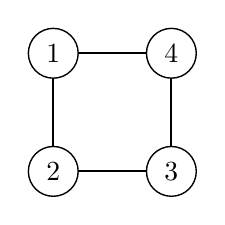
\begin{tikzpicture}[baseline=(current bounding box.center)]
          % vertices
          \Vertex[x=0,y=0,L=$1$]{1}
          \Vertex[x=1.5,y=0,L=$4$]{2}
          \Vertex[x=1.5,y=-1.5,L=$3$]{3}
          \Vertex[x=0,y=-1.5,L=$2$]{4}
          % edges
          \Edge(1)(2)
          \Edge(2)(3)
          \Edge(3)(4)
          \Edge(4)(1)
        \end{tikzpicture}
      \end{subfigure}
      %
      \Large$\Rightarrow$\normalsize\makebox[.2\paperwidth]{$\ (2\ 4)$\hfill}
    \end{figure}
  }
\end{frame}

% TODO: use picture instead
\begin{frame}
  \frametitle{Group Orbits}

  \begin{definition}
    We define the \textbf{orbit} of some $x \in \Omega$ under $G$ as:
    %
    \begin{equation*}
      x^G = \{g(x) \mid g \in G\}
    \end{equation*}
  \end{definition}
\end{frame}

\begin{frame}
  \frametitle{Representing Partial Symmetries:\\Partial Automorphism Inverse Monoids}

  \begin{figure}
    \centering
    %
    \begin{subfigure}{.2\paperwidth}
      \centering
      %
      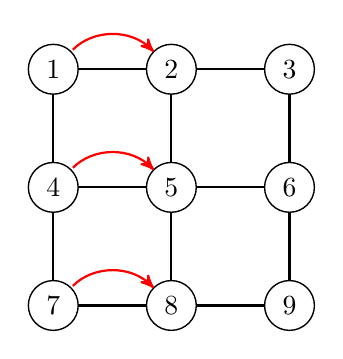
\begin{tikzpicture}[baseline=(current bounding box.center)]
        % vertices
        \Vertex[x=0,y=0,L=$1$]{1}
        \Vertex[x=1.5,y=0,L=$2$]{2}
        \Vertex[x=3,y=0,L=$3$]{3}
        \Vertex[x=0,y=-1.5,L=$4$]{4}
        \Vertex[x=1.5,y=-1.5,L=$5$]{5}
        \Vertex[x=3,y=-1.5,L=$6$]{6}
        \Vertex[x=0,y=-3,L=$7$]{7}
        \Vertex[x=1.5,y=-3,L=$8$]{8}
        \Vertex[x=3,y=-3,L=$9$]{9}
        % horizontal edges
        \Edge(1)(2)
        \Edge(2)(3)
        \Edge(4)(5)
        \Edge(5)(6)
        \Edge(7)(8)
        \Edge(8)(9)
        % vertical edges
        \Edge(1)(4)
        \Edge(2)(5)
        \Edge(3)(6)
        \Edge(4)(7)
        \Edge(5)(8)
        \Edge(6)(9)
        % arrows
        \tikzstyle{EdgeStyle}=[post, bend angle=45, bend left, style=thick]
        \Edge[color=red](1)(2)
        \Edge[color=red](4)(5)
        \Edge[color=red](7)(8)
      \end{tikzpicture}
    \end{subfigure}
    %
    \qquad\qquad\Large$\Rightarrow$\normalsize$\ [1\ 2][4\ 5][7\ 8]$
  \end{figure}
\end{frame}

\begin{frame}
  \frametitle{Extracting (Partial) Symmetries}

  \begin{itemize}
    \setlength\itemsep{.25cm}

    \item<1-> Describe MPSoC architecture as \textbf{architecture graph}

    \item<2-> Determine PG generating set:
      \begin{itemize}
        \item<3-> Transform into ``equivalent'' vertex colored graph
        \item<4-> Use \textit{nauty}~\cite{nauty}
      \end{itemize}
    \item<5-> Determine PPIM generating set:
      \begin{itemize}
        \item<6-> Construct search tree of possible generators
        \item<7-> Prune certain subtrees
        \item<8-> Not efficient enough in practice
      \end{itemize}
  \end{itemize}
\end{frame}

\begin{frame}
  \frametitle{Extracting (Partial) Symmetries}

  \only<1>{
    \begin{figure}
      \centering
      %
      \begin{subfigure}{.55\textwidth}
        \centering
        \includeressource[width=.8\textwidth]{simple_arch.pdf}
      \end{subfigure}
      %
      \Large$\Rightarrow$\normalsize
      %
      \begin{subfigure}{.3\textwidth}
        \centering
        %
        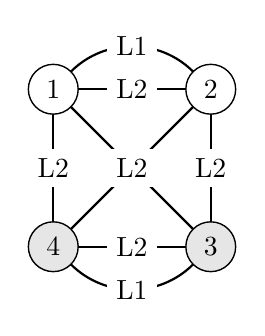
\begin{tikzpicture}
          % vertices
          \Vertex[x=0,y=0,L=$1$]{1}
          \Vertex[x=2,y=0,L=$2$]{2}
          {\renewcommand{\VertexLightFillColor}{LightGray}
           \Vertex[x=2,y=-2,L=$3$]{3}
           \Vertex[x=0,y=-2,L=$4$]{4}}
          % L2 edges
          \Edge[label=L2](1)(2)
          \Edge[label=L2](1)(3)
          \Edge[label=L2](1)(4)
          \Edge[label=L2](2)(3)
          \Edge[label=L2](2)(4)
          \Edge[label=L2](3)(4)
          % L1 edges
          \tikzstyle{EdgeStyle}=[bend angle=45, bend left]
          \Edge[label=L1](1)(2)
          \Edge[label=L1](3)(4)
        \end{tikzpicture}
      \end{subfigure}
    \end{figure}
  }

  \only<2>{
    \begin{figure}
      \centering
      %
      \begin{subfigure}{.3\textwidth}
        \centering
        %
        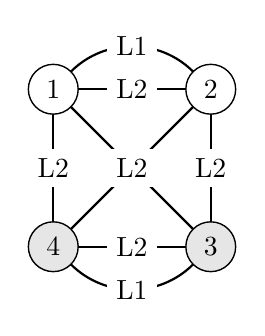
\begin{tikzpicture}
          % vertices
          \Vertex[x=0,y=0,L=$1$]{1}
          \Vertex[x=2,y=0,L=$2$]{2}
          {\renewcommand{\VertexLightFillColor}{LightGray}
           \Vertex[x=2,y=-2,L=$3$]{3}
           \Vertex[x=0,y=-2,L=$4$]{4}}
          % L2 edges
          \Edge[label=L2](1)(2)
          \Edge[label=L2](1)(3)
          \Edge[label=L2](1)(4)
          \Edge[label=L2](2)(3)
          \Edge[label=L2](2)(4)
          \Edge[label=L2](3)(4)
          % L1 edges
          \tikzstyle{EdgeStyle}=[bend angle=45, bend left]
          \Edge[label=L1](1)(2)
          \Edge[label=L1](3)(4)
        \end{tikzpicture}
      \end{subfigure}
      %
      \Large$\Rightarrow$\normalsize
      %
      \begin{subfigure}{.55\textwidth}
        \centering
        %
        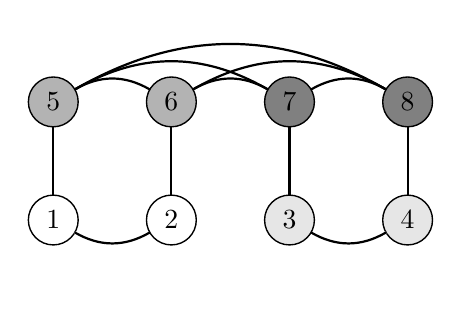
\begin{tikzpicture}
          % vertices
          \Vertex[x=0,y=-1.5,L=$1$]{1}
          \Vertex[x=1.5,y=-1.5,L=$2$]{2}
          {\renewcommand{\VertexLightFillColor}{LightGray}
            \Vertex[x=3,y=-1.5,L=$3$]{3}
            \Vertex[x=4.5,y=-1.5,L=$4$]{4}}
          {\renewcommand{\VertexLightFillColor}{MediumGray}
            \Vertex[x=0,y=0, L=$5$]{5}
            \Vertex[x=1.5,y=0, L=$6$]{6}}
          {\renewcommand{\VertexLightFillColor}{DarkGray}
            \Vertex[x=3,y=0, L=$7$]{7}
            \Vertex[x=4.5,y=0, L=$8$]{8}}
          % straight edges
          \Edge(1)(5)
          \Edge(2)(6)
          \Edge(3)(7)
          \Edge(4)(8)
          % dummy edge
          \tikzstyle{EdgeStyle}=[bend right]
          \Edge[color=white](1)(4)
          % bent edges
          \tikzstyle{EdgeStyle}=[bend right]
          \Edge(1)(2)
          \Edge(3)(4)
          \tikzstyle{EdgeStyle}=[bend left]
          \Edge(5)(6)
          \Edge(5)(7)
          \Edge(5)(8)
          \Edge(6)(7)
          \Edge(6)(8)
          \Edge(7)(8)
        \end{tikzpicture}
      \end{subfigure}
    \end{figure}
  }

  \only<3->{
    \begin{figure}
      \centering
      %
      \begin{subfigure}{.4\paperwidth}
        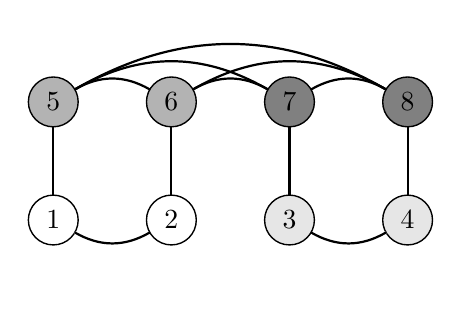
\begin{tikzpicture}
          % vertices
          \Vertex[x=0,y=-1.5,L=$1$]{1}
          \Vertex[x=1.5,y=-1.5,L=$2$]{2}
          {\renewcommand{\VertexLightFillColor}{LightGray}
            \Vertex[x=3,y=-1.5,L=$3$]{3}
            \Vertex[x=4.5,y=-1.5,L=$4$]{4}}
          {\renewcommand{\VertexLightFillColor}{MediumGray}
            \Vertex[x=0,y=0, L=$5$]{5}
            \Vertex[x=1.5,y=0, L=$6$]{6}}
          {\renewcommand{\VertexLightFillColor}{DarkGray}
            \Vertex[x=3,y=0, L=$7$]{7}
            \Vertex[x=4.5,y=0, L=$8$]{8}}
          % straight edges
          \Edge(1)(5)
          \Edge(2)(6)
          \Edge(3)(7)
          \Edge(4)(8)
          % dummy edge
          \tikzstyle{EdgeStyle}=[bend right]
          \Edge[color=white](1)(4)
          % bent edges
          \tikzstyle{EdgeStyle}=[bend right]
          \Edge(1)(2)
          \Edge(3)(4)
          \tikzstyle{EdgeStyle}=[bend left]
          \Edge(5)(6)
          \Edge(5)(7)
          \Edge(5)(8)
          \Edge(6)(7)
          \Edge(6)(8)
          \Edge(7)(8)
        \end{tikzpicture}
      \end{subfigure}
      %
      \Large$\Rightarrow$\normalsize\makebox[.3\paperwidth]{%
        $\ \{(1\ 2)$\st{$(5\ 6)$}$,(3\ 4)$\st{$(7\ 8)$}$\}$\hfill}
    \end{figure}
  }
\end{frame}

% TODO: use picture instead
\begin{frame}
  \frametitle{The TMOR Problem I:\\Mapping Orbits}

  \begin{itemize}
    \setlength\itemsep{.25cm}

    \item<1-> Represent mappings by $k$-tuples $t = (t_1, t_2, \dots, t_k)$
    \item<2-> Define space of all admissible $k$-mappings $\Theta_k$
    \item<3-> Define $t^G = \{((g(t_1), g(t_2), \dots, g(t_k))
          \mid g \in G\}$
    \item<4-> Orbits \textbf{partition} $\Theta_k$
    \item<5-> Reduce $\Theta_k$ to set of \textit{canonical orbit representatives}
  \end{itemize}
\end{frame}

\begin{frame}
  \frametitle{The TMOR Problem I:\\Mapping Orbits}

  \begin{itemize}
    \setlength\itemsep{.25cm}

    \item<1-> Determining all orbits usually too costly
    \item<2-> Iteratively determine and hash canonical representatives
  \end{itemize}

  \vspace{.25cm}

  \visible<3>{
    \begin{algorithmic}[1]
    \Procedure{ORBIT\_IDENTIFIER}{$t$, $\mathrm{reprs}$}
      \State $\mathrm{repr} \gets \mathrm{TMOR}(t)$
      \\
      \If{$\mathrm{repr} \notin \mathrm{reprs}$}
        \State Append $\mathrm{repr}$ to $\mathrm{reprs}$
      \EndIf
      \\
      \State \textbf{return} index of $\mathrm{repr}$ in $\mathrm{reprs}$
    \EndProcedure
    \end{algorithmic}
  }
\end{frame}

\begin{frame}
  \frametitle{The TMOR Problem II:\\Finding Canonical Orbit Representatives}

  \begin{itemize}
    \item First approach: explicit orbit enumeration
  \end{itemize}

  \vspace{.25cm}

  \begin{algorithmic}[1]
  \Procedure{TMOR\_ORBIT}{$t$, $G = \langle S \rangle$}
    \State $\mathrm{orbit} \gets \{\}$
    \\
    \While{$\mathrm{orbit}$ is changing}
      \For{$t' \in \mathrm{orbit}$, $g$ in $S$}
        \State $\mathrm{orbit} \gets \mathrm{orbit} \cup \{g(t')\}$
      \EndFor
    \EndWhile
    \\
    \State \textbf{return} $\min(\mathrm{orbit})$
  \EndProcedure
  \end{algorithmic}
\end{frame}

\begin{frame}
  \frametitle{The TMOR Problem II:\\Finding Canonical Orbit Representatives}

  \begin{itemize}
    \item Second approach: group enumeration
  \end{itemize}

  \vspace{.25cm}

  \begin{algorithmic}[1]
  \Procedure{TMOR\_ITERATE}{$t$, $G$}
    \State $\mathrm{repr} \gets t$
    \\
    \For{$g \in G$}
      \If{$g(t) < \mathrm{repr}$}
        \State $\mathrm{repr} \gets g(t)$
      \EndIf
    \EndFor
    \\
    \State \textbf{return} $\mathrm{repr}$
  \EndProcedure
  \end{algorithmic}
\end{frame}

\begin{frame}
  \frametitle{The TMOR Problem II:\\Finding Canonical Orbit Representatives}

  \begin{itemize}
    \item Third approach: local search
  \end{itemize}

  \vspace{.25cm}

  \begin{algorithmic}[1]
  \Procedure{TMOR\_LOCAL\_SEARCH}{$t$, $G = \langle S \rangle$}
    \State $\mathrm{repr} \gets t$
    \\
    \While{$\mathrm{repr}$ is changing}
      \State $\mathrm{repr} \gets \min(\{g(\mathrm{repr}) \mid g \in S\})$
    \EndWhile
    \\
    \State \textbf{return} $\mathrm{repr}$
  \EndProcedure
  \end{algorithmic}
\end{frame}

\begin{frame}
  \frametitle{The TMOR Problem III:\\Optimization by Decomposition}

  \begin{itemize}
    \setlength\itemsep{.25cm}

    \item<1-> Many architecture graphs are \textit{separable} or
          \textit{hierarchical}
    \item<2-> Separable: any heterogeneous archictecture
    \item<3-> Hierarchical: \textbf<3>{HAEC}\visible<4->{, \textbf{Kalray}}
  \end{itemize}

  \vspace{.25cm}

  \visible<3->{
    \begin{figure}
      \centering
      \begin{overprint}
        \onslide<3>\centerline{\includeressource[width=.4\textwidth]{haec.pdf}}
        \onslide<4>\centerline{\includeressource[width=.8\textwidth]{kalray.pdf}}
      \end{overprint}
    \end{figure}
  }
\end{frame}

\begin{frame}
  \frametitle{The TMOR Problem III:\\Optimization by Decomposition}

  \begin{itemize}
    \setlength\itemsep{.25cm}

    \item<1-> Automorphism groups of such graphs decompose into:
      \begin{itemize}
        \setlength\itemsep{.25cm}

        \item<2-> Separable architectures: \textit{direct products}\\
              $G = G_1 \times G_2$, $|G| = |G_1| \cdot |G_2| \cdots |G_n|$
        \item<3-> Hierarchical architectures: \textit{wreath products}\\
              $G = G_{\mathrm{proto}} \wr G_{\mathrm{super}}$,
              $|G| = |G_{\mathrm{proto}}|^{\operatorname{deg}(G_{\mathrm{super}})}
               \cdot |G_{\mathrm{super}}|$
      \end{itemize}
    \item<4-> Decomposition specified by user or detected automatically
    \item<5-> Solve TMOR problem separately for components
    \item<6-> Idea based on~\cite{Donaldson}
  \end{itemize}
\end{frame}

\begin{frame}
  \frametitle{The TMOR Problem III:\\Optimization by Decomposition}

  \begin{itemize}
    \item For separable architectures:
  \end{itemize}

  \vspace{.25cm}

  \begin{algorithmic}[1]
    \Procedure{TMOR\_SEPARABLE}{$t$, $G_1, \dots, G_n$}
      \State $\mathrm{repr} \gets t$
      \\
      \For{$i = 1 \dots n$}
        \State $\mathrm{repr} \gets \mathrm{TMOR}(\mathrm{repr}, G_i)$
      \EndFor
      \\
      \State \textbf{return} $\mathrm{repr}$
    \EndProcedure
  \end{algorithmic}
\end{frame}

\begin{frame}
  \frametitle{The TMOR Problem III:\\Optimization by Decomposition}

  \begin{itemize}
    \item For hierarchical architecture:
  \end{itemize}

  \vspace{.25cm}

  \begin{algorithmic}[1]
  \Procedure{TMOR\_HIERARCHICAL}{$t$, $G_{\mathrm{proto}}$, $G_{\mathrm{super}}$}
    \State $\mathrm{repr} \gets t$
    \\
    \For{$i = 1 \dots \operatorname{deg}(G_{\operatorname{super}})$}
      \State $\mathrm{repr} \gets \mathrm{TMOR}(\mathrm{repr},
                                                \sigma_i(G_{\mathrm{proto}}))$
    \EndFor
    \\
    \State \textbf{return} $\mathrm{TMOR}(\mathrm{repr}, \sigma(G_{\mathrm{super}}))$
  \EndProcedure
  \end{algorithmic}
\end{frame}

\begin{frame}
  \frametitle{Experimental Results I:\\Architectures}

  \begin{itemize}
    \item Experiments run for:
          \textbf<1>{Exynos}
          \visible<2->{, \textbf<2>{Parallella}}
          \visible<3->{, \textbf<3>{HAEC}}
          \visible<4->{, \textbf<4>{Kalray}}
  \end{itemize}

  \vspace{.25cm}

  \begin{overprint}
    \onslide<1>\centerline{\includeressource[width=.4\textwidth]{exynos.pdf}}
    \onslide<2>\centerline{\includeressource[width=.4\textwidth]{parallella.pdf}}
    \onslide<3>\centerline{\includeressource[width=.5\textwidth]{HAEC.pdf}}
    \onslide<4>\centerline{\includeressource[width=.8\textwidth]{Kalray.pdf}}
  \end{overprint}
\end{frame}

\begin{frame}
  \frametitle{Experimental Results II:\\BSGS Construction}

  \begin{figure}
    \centering
    \scalebox{.7}{\inputressource{bsgs_boxplot.tex}}
  \end{figure}
\end{frame}

\begin{frame}
  \frametitle{Experimental Results II:\\BSGS Construction}

  \begin{itemize}
    \item<1-> Finding BSGS for $G_{\mathrm{Kalray}}$ too expensive:
      \begin{itemize}
        \setlength\itemsep{.25cm}

        \item<2-> Only construct BSGS for $G_{\mathrm{Kalray,proto}}$,
                  $G_{\mathrm{Kalray,super}}$
        \item<3-> Detect symmetric automorphism group
        \item<4-> Improvement from several minutes to $\approx 10^{-1}s$
      \end{itemize}
  \end{itemize}
\end{frame}

\begin{frame}
  \frametitle{Experimental Results II:\\TMOR}

  \scalebox{.7}{\inputressource{exynos_lineplot.tex}}
\end{frame}

\begin{frame}
  \frametitle{Experimental Results II:\\TMOR}

  \scalebox{.7}{\inputressource{parallella_lineplot.tex}}
\end{frame}

\begin{frame}
  \frametitle{Experimental Results II:\\TMOR}

  \scalebox{.7}{\inputressource{haec_lineplot.tex}}
\end{frame}

\begin{frame}
  \frametitle{Experimental Results II:\\TMOR}

  \scalebox{.7}{\inputressource{haec_histogram.tex}}
\end{frame}

\begin{frame}
  \frametitle{Experimental Results II:\\TMOR}

  \scalebox{.7}{\inputressource{kalray_lineplot.tex}}
\end{frame}

\begin{frame}
  \frametitle{Experimental Results II:\\TMOR}

  \begin{itemize}
    \item Lessons learned:
      \begin{itemize}
        \setlength\itemsep{.25cm}

        \item<1-> Performance of orbit enumeration depends strongly on $k$
        \item<2-> Local search can be fast and accurate
        \item<3-> Decomposition can be very powerful
        \item<4-> \texttt{mpsym} outperforms GAP
      \end{itemize}
  \end{itemize}
\end{frame}

\begin{frame}
  \frametitle{The End}

  \begin{center}
    Thank you for your attention!
  \end{center}
\end{frame}

\begin{frame}
  \frametitle{Further Research}

  \begin{itemize}
    \setlength\itemsep{.25cm}

    \item<1-> Faster BSGS Construction
    \item<2-> Heuristic local search
    \item<3-> Partial Automorphism discovery
    \item<4-> Inverse Monoid enumeration
    \item<5-> Compiling GAP to C
  \end{itemize}
\end{frame}

\begin{frame}
  \frametitle{References}

  \tiny

  \bibliography{bibliography}
  \bibliographystyle{apalike}
\end{frame}

\end{document}
